\documentclass[tikz, 12pt]{report}
\usepackage[utf8]{inputenc}
\usepackage[margin=20mm]{geometry}
\usepackage[pdfborder={0 0 0},backref=page]{hyperref}
\usepackage{dissertation}
\usepackage{lineno}
\linespread{1.5}

\hypersetup{
    colorlinks=true,
    urlcolor=blue,
    linkcolor=black,
    citecolor=blue!70!black,
}

\bibliographystyle{apalike}

\title{{ \includegraphics[scale=.5]{figures/ucl_logo.png}}\\
{{\Huge Does Size Matter?}\\{\Large The Effect of Sample Size on Steering}}\\
}
\date{Submission date: 8 September 2025}
\author{PRHC8\thanks{
{\bf Disclaimer:}
This report is submitted as part requirement for the Machine Learning MSc at UCL. It is
substantially the result of my own work except where explicitly indicated in the text.
The report may be freely copied and distributed provided the source is explicitly acknowledged}
\\ \\
Machine Learning MSc\\ \\
Daniel Tan \& Brooks Paige}

\begin{document}
\linenumbers

%TC:ignore
%%%%% NEW MATH DEFINITIONS %%%%%

% Mark sections of captions for referring to divisions of figures
\newcommand{\figleft}{\em (Left)}
\newcommand{\figcenter}{\em (Center)}
\newcommand{\figright}{\em (Right)}
\newcommand{\figtop}{\em (Top)}
\newcommand{\figbottom}{\em (Bottom)}
\newcommand{\captiona}{\em (a)}
\newcommand{\captionb}{\em (b)}
\newcommand{\captionc}{\em (c)}
\newcommand{\captiond}{\em (d)}

% Highlight a newly defined term
\newcommand{\newterm}[1]{\mathbf #1}

\def\ceil#1{\lceil #1 \rceil}
\def\floor#1{\lfloor #1 \rfloor}
\def\1\mathbf{1}
\newcommand{\train}{\mathcal{D}}
\newcommand{\valid}{\mathcal{D\_\mathrm{valid}}}
\newcommand{\test}{\mathcal{D\_\mathrm{test}}}

\def\eps{\epsilon}

% Vectors
\def\vzero{\mathbf{0}}
\def\vone{\mathbf{1}}
\def\vmu{\mathbf{\mu}}
\def\vtheta{\mathbf{\theta}}
\def\va{\mathbf{a}}
\def\vb{\mathbf{b}}
\def\vc{\mathbf{c}}
\def\vd{\mathbf{d}}
\def\ve{\mathbf{e}}
\def\vf{\mathbf{f}}
\def\vg{\mathbf{g}}
\def\vh{\mathbf{h}}
\def\vi{\mathbf{i}}
\def\vj{\mathbf{j}}
\def\vk{\mathbf{k}}
\def\vl{\mathbf{l}}
\def\vm{\mathbf{m}}
\def\vn{\mathbf{n}}
\def\vo{\mathbf{o}}
\def\vp{\mathbf{p}}
\def\vq{\mathbf{q}}
\def\vr{\mathbf{r}}
\def\vs{\mathbf{s}}
\def\vt{\mathbf{t}}
\def\vu{\mathbf{u}}
\def\vv{\mathbf{v}}
\def\vw{\mathbf{w}}
\def\vx{\mathbf{x}}
\def\vy{\mathbf{y}}
\def\vz{\mathbf{z}}

% Matrix
\def\mA{\mathbf{A}}
\def\mB{\mathbf{B}}
\def\mC{\mathbf{C}}
\def\mD{\mathbf{D}}
\def\mE{\mathbf{E}}
\def\mF{\mathbf{F}}
\def\mG{\mathbf{G}}
\def\mH{\mathbf{H}}
\def\mI{\mathbf{I}}
\def\mJ{\mathbf{J}}
\def\mK{\mathbf{K}}
\def\mL{\mathbf{L}}
\def\mM{\mathbf{M}}
\def\mN{\mathbf{N}}
\def\mO{\mathbf{O}}
\def\mP{\mathbf{P}}
\def\mQ{\mathbf{Q}}
\def\mR{\mathbf{R}}
\def\mS{\mathbf{S}}
\def\mT{\mathbf{T}}
\def\mU{\mathbf{U}}
\def\mV{\mathbf{V}}
\def\mW{\mathbf{W}}
\def\mX{\mathbf{X}}
\def\mY{\mathbf{Y}}
\def\mZ{\mathbf{Z}}
\def\mBeta{\mathbf{\beta}}
\def\mPhi{\mathbf{\Phi}}
\def\mLambda{\mathbf{\Lambda}}
\def\mSigma{\mathbf{\Sigma}}

% Sets
\def\sA{\mathcal{A}}
\def\sB{\mathcal{B}}
\def\sC{\mathcal{C}}
\def\sD{\mathcal{D}}
\def\sE{\mathcal{E}}
\def\sF{\mathcal{F}}
\def\sG{\mathcal{G}}
\def\sH{\mathcal{H}}
\def\sI{\mathcal{I}}
\def\sJ{\mathcal{J}}
\def\sK{\mathcal{K}}
\def\sL{\mathcal{L}}
\def\sM{\mathcal{M}}
\def\sN{\mathcal{N}}
\def\sO{\mathcal{O}}
\def\sP{\mathcal{P}}
\def\sQ{\mathcal{Q}}
\def\sR{\mathcal{R}}
\def\sS{\mathcal{S}}
\def\sT{\mathcal{T}}
\def\sU{\mathcal{U}}
\def\sV{\mathcal{V}}
\def\sW{\mathcal{W}}
\def\sX{\mathcal{X}}
\def\sY{\mathcal{Y}}
\def\sZ{\mathcal{Z}}

\newcommand{\E}{\mathbb{E}}
\newcommand{\Ls}{\mathcal{L}}
\newcommand{\R}{\mathbb{R}}
\newcommand{\N}{\mathbb{N}}
\newcommand{\emp}{\tilde{p}}
\newcommand{\lr}{\alpha}
\newcommand{\reg}{\lambda}
\newcommand{\rect}{\mathrm{rectifier}}
\newcommand{\softmax}{\mathrm{softmax}}
\newcommand{\sigmoid}{\sigma}
\newcommand{\softplus}{\zeta}
\newcommand{\KL}{D\_\mathrm{KL}}
\newcommand{\Var}{\mathrm{Var}}
\newcommand{\standarderror}{\mathrm{SE}}
\newcommand{\Cov}{\mathrm{Cov}}
% Wolfram Mathworld says $L^2$ is for function spaces and $\ell^2$ is for vectors
% But then they seem to use $L^2$ for vectors throughout the site, and so does
% wikipedia.
\newcommand{\normlzero}{L\^0}
\newcommand{\normlone}{L\^1}
\newcommand{\normltwo}{L\^2}
\newcommand{\normlp}{L\^p}
\newcommand{\normmax}{L\^\infty}

\newtheorem{theorem}{THEOREM}
\newtheorem{lemma}[theorem]{LEMMA}
\newtheorem{corollary}[theorem]{COROLLARY}
\newtheorem{proposition}[theorem]{PROPOSITION}
\newtheorem{remark}[theorem]{REMARK}
\newtheorem{definition}[theorem]{DEFINITION}
\newtheorem{fact}[theorem]{FACT}

\newtheorem{problem}[theorem]{PROBLEM}
\newtheorem{exercise}[theorem]{EXERCISE}
\def \set#1{\{#1\} }

\newenvironment{proof}{
PROOF:
\begin{quotation}}{
$\Box$ \end{quotation}}

\newcommand{\mfullname}{Skye Purchase}
\newcommand{\mtitle}{As Yet Untitled}
\newcommand{\mdate}{\today}
\newcommand{\msupervisor}{}


\pagenumbering{roman}

\onehalfspacing
\maketitle

\chapter*{Acknowledgements}

I want to thank my family, especially my mum and dad who have supported me throughout my life and encouraged me to explore the world.
To my wider family who have both directly and indirectly supported me throughout the masters.

Particular thanks goes to Mia who has supported me throughout the highs and lows, stress and anxiety of the masters and the year leading up to it.
Thank you for listening to my endless rambles about the project and all the other projects I've had; keeping me focused, motivated, and on track to complete the thesis.

I would like to thank my supervisor Daniel Tan and the support of the ML Alignment and Theory Scholars London office for guiding the project and providing feedback along the way.
Additionally, to Alex for providing detailed, actionable feedback on my early rough drafts.

\begin{abstract}
Summarise your report concisely.
\end{abstract}

\tableofcontents
\listoffigures
\listoftables
\clearpage
\pagenumbering{arabic}
%TC:endignore

\chapter{Introduction}
\label{ch:introduction}

\emph{In this chapter an overview of the project and this report is detailed.}
\emph{This includes what the project involves as well as why this is a worthwhile project.}
\emph{The motivation for the project will be briefly discussed along with the benefits of the analysis carried out.}

\emph{Related work to this project, including projects which precede this one and projects which cover separate but related issues, is presented.}
\emph{The differences between this project and the related work is explained.}

\emph{Finally the contributions which this project make to the field are detailed.}
\emph{These contributions are justified in \cref{ch:results} and reiterated in \cref{ch:conclusion}.}

\section{Motivation}

In recent years the use of machine learning (ML) models has rapidly increased across multiple sectors of life.
In particular the rise in deep learning models following the release of Alexnet \citep{alexnet} has introduced new problems with the use of ML.
This has lead to rapid development in field resulting  model capabilities surpassing human capabilities in an increasing range of activities \citep{dynabench, gpt-5, grok-4, hle}.
With the introduction of large language model (LLM) chatbots starting with ChatGPT \citep{chatgpt}, ML models are increasingly becoming part of everyday life.

There are already cases of serious harm to users \citep{c.ai, psychosis} and the potential for humanity scale risk posed by increasingly capable systems has been posed \citep{survellience, deepfakes, disempowerment}.
There are many approaches to try and solve these problems ranging from law and policy to model training techniques and dataset design.

The field of preventing risks posed by ML is known as AI (artificial intelligence) safety.
A primary goal of AI safety is to alter models to be more ``helpful'', ``honest'', and ``harmless'' without effecting their performance.
A promising avenue of AI safety, especially for LLMs, is \emph{steering adaptors} a subset of representation engineering \citep{steering-taxonomy}.
The basic concept behind steering adaptors is to \emph{manipulate the internal representation space} of models.
By assuming certain \emph{directions within representation space represent understandable concepts} it is possible to perturb a models vector representation towards a target concept.
This idea has already been demonstrated by \citet{word2vec} in word embedding models.

There is large amounts of anecdotal evidence of steering adaptors successfully changing model behaviour with increasing studies looking into the theory \citep{steering-clear, steering-theory} and effectiveness \citep{steerability, steering-taxonomy} of steering adaptors on modern models.
There, however, continue to be a lack of large scale studies comparing a range of adaptors in realistic settings with varying input size and hyperparameter choice.

This project and report aim to remedy this and provide more quantitative and qualitative analysis of common steering techniques on LLMs.
The project will hopefully provide insight into the effectiveness of these techniques as well as the suitability of a selection of suggested metrics.

\subsection{Benefits of Steering Vectors}

Unlike other techniques to change a models behaviour such as reinforcement learning \citep{rl, rlhf} or finetuning \citep{lora} steering adaptors require far less compute and data as they do not require changing the many parameters of the chosen model.
Once implemented they are efficient to run during inference and have been shown to have low impact on model capabilities \citep{steering-wo-ss, sea}.
Importantly, these techniques are still compatible with other alignment techniques working to provide additional adjustments.

By nature they inherently provide some interpretability by demonstrating how certain model representations effect the output.
This, in turn, allows for more precise control over model behaviour than other techniques with potential direct feedback between the user and the model behaviour.
However, these techniques frequently require full access to the model's parameters and architecture.

\section{Research Questions}
\label{sec:questions}

This project aims to provide a detailed, quantitative comparison of steering adaptors in realistic settings.
This work follows the work on analysing the generalisability of steering vectors in \citet{steerability} and the survey of current representation engineering techniques from \citet{steering-taxonomy}.
The approach used in this project extends the analysis of steering example size on adaptor performance in the toy setting proposed by \citet{steering-clear} to the natural language setting using LLMs.
Furthermore, a comparison of the new affine concept editing \citep[ACE]{ace} adaptor is made against existing adaptors.
The three research questions therefore focus on reproducing prior results and providing new results and analysis.

\begin{enumerate}[nolistsep]
    \item Are the findings of \citet{steering-clear} reproducible and sound? Where does the adaptor proposed by \citet{ace} fit into their analysis?
    \item How do the number of examples effect the performance of steering adaptors? Does this match the results in the toy setting of \citet{steering-clear}? What metrics provide meaningful insight into steering performance?
    \item How can the success of steering adaptors be quantified in the natural language setting?
\end{enumerate}

Overall this projects aims to provide more insight into when steering methods work focusing on the number of steering examples.
Additional discussion on the shortcomings of the steering approaches are provided throughout as well as suggestions for real world use.

\section{Compute Environment}

The project was written and programmed on my personal laptop.
This is a Dell Inspiron 15'' laptop running Arch Linux and i3 window manager.
The laptop has 16GB of memory with an 8 core Intel 13$^{th}$ generation i7 processor.

Preliminary tests of the experiments run in this project were done on this laptop.
However, the official results were run on \href{https://www.runpod.io/}{RunPod}, which provides a suite of possible GPU environments.
For all the results presented in \cref{ch:results} the RTX 2000 Ada environment was used.
This environment includes a single RTX 2000 Ada GPU with 16GB of VRAM, 31GB of RAM, and 6 virtual CPUs.
The cost to run this environment was \$0.24 per hour.
The funding for the compute environment was provided by my supervisor through the \href{https://www.matsprogram.org/}{ML Alignment and Theory Scholarship} which he is part of.

Occasional use of the free \href{https://colab.research.google.com/}{Google Colab} environment was used to verify the experiments ran at scale.
No results presented in this report were generated from these runs.

\section{Generative AI Disclosure}

This project aims to steer generative AI models (genAI) such as GPT 2 \citep{gpt-2} and thus genAI was used in generating the raw results presented in \cref{ch:results}.

However, outside of the direct prompting of agents to analyse the steering adaptors presented in \cref{ch:background}, no generative AI was used throughout the project or report.
There are two exceptions:
\begin{itemize}[nolistsep]
    \item Generating a dataset of prompt-completion templates detailed in \cref{app:prompt-pairs}.
    \item Generating a random point cloud in Tikz for \cref{fig:caa}.
\end{itemize}

Spellcheck was performed by Neovim and its built in spellchecker with no use of AI tools such as Grammarly.
All citations were found and generated through Google Scholar.
Assistance for Tikz diagrams was found through \href{https://www.tikz.dev}{https://www.tikz.dev}.

However, with the proliferation of AI in search engines it is not possible to state that genAI did not influence any of the \LaTeX~or code snippets.
I endeavoured to not use genAI as much as possible throughout the last 3 months.

\section{Related Work}

\smalltitle{\citet{steering-clear}}
aim to analyse steering in a toy environment where they are able to control the representation density within the model.
They compare a range of steering techniques \citep{caa, reft, mimic} against each other in a controlled setting to focus on the effect of steering example size.
Inspired by the low-rank representation finetuning \citep[LoReFT]{reft} (A steering adaptor which steers representations in a projected, low-rank space) they introduce their own technique, low-rank representation steering (LoReST), and demonstrate competitive performance to the other techniques.

To verify this work, this thesis reproduces the same toy environment described in \cref{sec:steering-clear} and validates the conclusions drawn.
Additionally, this reproduction introduces the affine concept editing adaptor proposed by \citet{ace} to compare against the adaptors used in \citet{steering-clear}.
This thesis then expands the analysis to LLMs and demonstrates similar adaptor performance in relation to the number of training examples suggesting the same preference for low-rank methods in the large data regime and affine methods in the small data regime.
Furthermore, this thesis shows the consistency of LoReST in both data regimes.

\smalltitle{\citet{steerability}}
analyse the generalisation of steering vectors across a range of steering datasets.
They analyse the variability of success and introduce the notion of ``steerability''.
Using this notion they demonstrate that many techniques fail to generalise on certain datasets both in and out of distribution.

The analysis is limited to only contrastive activation addition \citep{caa} which \citet{steering-clear} show is not necessarily the ideal candidate.
Building on their work this project aims to analyse a larger range of techniques sampled from \citet{steering-clear}.
Furthermore, the properties of training datasets is analysed in more depth to determine which properties cause steering techniques to fail.

In this thesis, rather than use model written evaluations \citep{mwe} a new set of steering datasets is generated with more fine grain control.
The construction of these datasets is described in \cref{sec:prompt-pairs}.

\smalltitle{\citet{steering-taxonomy}}
present a full taxonomy of current steering vector approaches (more generally \emph{representation engineering}).
The paper covers a range of topics within representation engineering that have been carried out by the community.
These focus on the types of adaptors used, the prompting framework, linear vs. non-linear adaptors, the concepts that are steered, etc.

This thesis continues these comparisons by analysing the effect of the dataset and number of steering examples used in the large language model setting.
It is impractical to expand the experiments to all the approaches described in \citet{steering-taxonomy} due to time constraints so only those discussed in \citet{steering-clear} are analysed.


\smalltitle{Sparse autoencoders as steering vectors}
There are multiple papers that utilise sparse autoencoders (SAEs) as steering vectors \citep{sae-improved, sae-steering, icl-sae}.
SAEs work by transforming the dense model representations into a high-dimensional, sparse vector space.
This allows individual dimensions to represent unique, human-understandable concepts effectively ``decoding'' the model representation.
These approaches utilise this fact, that SAEs decode high level concepts from the models intermediate representation to steer the model towards or away from said concepts.
This process works by ``reversing'' the SAE procedure and converting concepts into potential representation perturbations.

This thesis, in contrast, uses the SAE features to evaluate models on free-text responses rather than utilising SAEs to steer the model.
The SAE features provide a metric to evaluate how well the models internal representation has been effectively steered.
A detailed description of SAEs is provided in \cref{sec:sae} and their use in this project is described in \cref{sec:prompt-pairs}.

\section{Contributions}
\label{sec:contributions}

In answering the questions posed in \cref{sec:questions} this project provides the following contributions
\begin{itemize}[nolistsep]
    \item Verification of the results presented by \citet{steering-clear} in their toy experiment.
    \item Comparison of contrastive activation addition \citep[CAA]{caa}, affine concept editing \citep[ACE]{ace}, LoReFT and LoReST on large language models.
    \item In depth analysis on the effect of the number of steering examples on the adaptor performance.
    \item A set of promising LLM steering metrics along with qualitative analysis of the steered model output.
\end{itemize}

All code for the project is available at \href{https://github.com/skyepurchase/msc_thesis}{this code repository} and all the \LaTeX~including diagrams is available at \href{https://github.com/skyepurchase/msc_report}{this, separate, code repository}.

\chapter{Background}
\label{ch:background}

\emph{In this chapter the notation, phrases and concepts that are used throughout the document are explained.}
\emph{An overview of general model alignment as well as the specifics of alignment via steering adaptors is described.}
\emph{This includes a history of the different techniques and the details of the four methods used in this project.}

\emph{The history of large language models and why they are important in current research is outline.}
\emph{Additionally the challenges that are faced in interpretting these large models is explained.}
\emph{The solutions to these challenges present possible metrics that can be used to analyse the effectiveness of steering adaptors.}

\section{Notation and Concepts}

Throughout this report ``neural network (NN)'' \Sref{sec:deep-learning} and ``machine learning (ML) model'' are used interchangeably though NNs are a strict subset of ML models.
In general the term ``model'' is used to refer to the collective group and represents any program that adjusts tunable parameters to predict output from input examples.

Model ``behaviours", in general, are patterns in how the model responds to input.
This includes the desired behaviour it was trained on (such as classifying images of cats and dogs) but includes patterns in the output that were not explicitly trained for.
Desired model behaviour is considered ``positive" and undesired model behaviour is considered ``negative".
Specifically, an example of the desired behaviour is considered a ``positive example'' and an example of undesired or neutral behaviour is considered a ``negative'' example.
An example of a behaviour generally includes an input-output pairing similar to training examples however they are more specific pairings than would be using during training.

When discussing NNs the concept of a ``neuron'' relates to the abstract structure that receives a real-valued, vector input and outputs a real-value scalar based on internal, learnable weights.
In practice, this is represented by a single element of a NN layer's output vector.
Furthermore, a \emph{module} refers to a collection of one or more NN layers.
A model may be made of multiple modules or be a single module.
Modules may be ``attached'' to specific layers within a model whereby the output of the layer is passed to the module as input and the module may augment, store, or monitor the data flow in the model.
These ideas are described and discussed in more detail in the deep learning section \Sref{sec:deep-learning}.

Vectors are represented by boldface letters, $\vx, \vy, \vz$, scalars are represented by greek letters, $\alpha, \beta, \gamma$, and matrices are represented by boldface capital letters, $\mA, \mB, \mC$.
Some matrices may represent transformations or collections of feature vectors, context should disambiguate the two.
In general vectors are column vectors, $\vx = \begin{bmatrix*}
    1 & 2 & \cdots & n
\end{bmatrix*}^T$ except when a collection of vectors is represented in matrix form, in this case each row is a vector.

In a multi-layer machine learning model the output of an internal layer is an ``activation'' denoted $\va$.
A positive activation is denoted $\va^+$ and a negative activation is denoted as $\va^-$. Here, ``positive activation'' means the activation extracted from the model given a positive example as above.
The mean of a set of activations, $\mathcal{A} = \{\va_i\}_{i < n}$, is denoted $\mu_\mathcal{A} = \frac{1}{n}\sum_{i=1}^{n}\va_i$.
Frequently the set of set of activations will be the positive activation or negative activation set, in this case the mean is denoted $\mu_{\va^+}$ or $\mu_{\va^-}$ respectively.

\section{Deep Learning}
\label{sec:deep-learning}

\section{Model Alignment}

As models increase in capabilities \citep{dynabench, hle, gpt-5, grok-4} they pose an increasing risk to their users \citep{c.ai, psychosis} and potentially humanity at large \citep{survellience, deepfakes, disempowerment}.
The underlying issue is that these models may be \emph{misaligned} \citep{agent-alignment}, that is to say they do not behaviour in line with users intentions.
The problem of aligning models is referred to as the \emph{alignment problem} or, within reinforcement learning \cite{rl}, the \emph{agent alignment problem} \citep{agent-alignment}.\footnote{An \emph{agent} is a reinforcement learning term for any entity that interacts with a learning environment and updates it's internal state to better achieve a predetermined goal. In this case, the model behaves as an agent.}

\citet{agent-alignment} present the agent alignment problem and propose \emph{reward modelling} as a potential avenue to align agents.
They outline a couple of assumptions as to whether reward modelling is suitable:
\begin{itemize}[nolistsep]
    \item It is possible to sufficiently learn user intentions.
    \item It is cheaper to evaluate outcomes than produce the ``correct'' behaviour.
\end{itemize}
Working on this, \citet{rlhf} apply these ideas to large language models (LLM)s.
The goal is to transform purely predictive LLMs into assistants that are ``helpful'', ``honest'', and ``harmless''.
This is achieved by utilising human feedback on LLM output as rewards for reward modelling.
This technique paved the way for the model AI chatbot \citep{chatgpt}.
The technique of reinforcement learning from human feedback (RLHF) had been developed previously by \citet{rlhf-orig} but had not been applied to LLMs.

RLHF has been shown to be very effective in transforming the behaviour of models.
However, it is still possible for RLHF ``aligned'' models to be misaligned \citep{misgeneralization, c.ai}.
Furthermore, this approach to alignment is very costly requiring human annotators, reviewers and the costly process of finetuning.
Techniques to mitigate this have been proposed including RLxF \citep{alignment-survey}, utilising both human and AI feedback, representation finetuning \citep{reft}, and parameter efficient finetuning \citep{peft}.

Representation finetuning or more generally representation engineering \citep{steering-taxonomy} presents a promising avenue for alignment \citep{steering-clear, steering-theory, steering-taxonomy}.
Rather than requiring large amounts of human annotated data and changing model weights only the representations need editting.
This thesis focuses on \emph{steering adaptors}, a subset of representation engineering.

\section{Steering Adaptors}

The general form of a steering adaptor is a simple module that augments a layer's output.
The idea is to change the internal representation away from a harmful or misaligned concept towards one that is aligned to the users intentions.
The goal is to keep all other aspects of the representation intact so that the performance of the model is not hindered.

Rather than large amounts of annotated data or large weight matrices these techniques require a handful of positive and negative examples.
Given their lightweight nature these techniques have shown promising results \citep{steering-taxonomy, steering-theory, steering-clear, reft}.

\subsection{Contrastive Activation Addition}
\label{caa}

An intuitative approach to model intervention is to perturb the model's activations in a desired direction.
By calculating a linear direction in activation space from undesired activations towards desired ones this vector can simply be added to all activations in the model during inference.
The hope is that the model produces output that matches the desired behaviour whilst maintaining the context of the new input.

\begin{figure}
    \centering
    \captionsetup{width=.9\textwidth}
    \begin{tikzpicture}

\foreach \i in {1,...,100} {
    % generate random coords and save them in dedicated macros
    \pgfmathsetmacro{\rr}{rnd*2}       % x in [0,6]
    \pgfmathsetmacro{\rtheta}{rnd*360}   % y in [-3,3]
    \node[red] at ({\rr*cos(\rtheta)},{\rr*sin(\rtheta)}) {$\times$};
}

% Second set (green crosses), horizontally shifted
\foreach \i in {1,...,100} {
    \pgfmathsetmacro{\rr}{rnd*2}       % x in [0,6]
    \pgfmathsetmacro{\rtheta}{rnd*360}   % y in [-3,3]
    \node[green!70!black] at ({7+\rr*cos(\rtheta)},{\rr*sin(\rtheta)}) {$\times$};
}

% Draw mean points
\node[circle, fill=red, inner sep=3pt, label={[yshift=4em,xshift=-4em]$\mu_{\va^-}$}] (meanA) at (0,0) {};
\node[circle, fill=green!70!black, inner sep=3pt, label={[yshift=4em,xshift=4em]$\mu_{\va^+}$}] (meanB) at (7,0) {};

% Draw dashed arrow between means
\draw[dashed, -{Stealth[length=3mm]}, thick] (meanA) -- (meanB)
    node[midway, above] {$\vv_{steer} = \mu_{\va^+} - \mu_{\va^-}$};

% Draw random point to steer
\node[rectangle, fill=black, inner sep=2pt] (test) at (1, 1) {};
\node[rectangle, fill=green!70!black, inner sep=2pt] (steered) at (8, 1) {};

% Draw dashed arrow between steered points
\draw[-{Stealth[length=3mm]}, thick] (test) -- (steered)
    node[midway, above] {$\va_{steer} = \va + \vv_{steered}$};

\end{tikzpicture}

\caption{Demonstration of contrastive activation addition \citep{caa}. The figure represents a simple representation space of dimension 2 with clear separability. $\mu_A = \frac{1}{\|A\|}\sum_{i \in \mathcal{I}(A)} A_i$ where $A$ is a set of activation vectors. A new point, such as the black square, is translated by the steering vector.}
    \label{fig:caa}
\end{figure}

In the simplest form consider two example inputs with desired and undesired behaviour.
Their difference gives a direction in feature space that corresponds to shifting the models output from undesired behaviour towards desired behaviour.
This is the approach proposed by \citet{activation-addition}, however, it is not robust and relies heavily on the example inputs \citep{caa}.

To improve on this approach \citet{caa} suggest using a collection of examples and calculating their mean difference in activation space.
This requires the notion of \textit{contrastive pairs}, two inputs that are similar in all ways except for the behaviour that is being changed.
Hence, this approach is known as \textit{contrastive activation addition} (CAA).
This process is demonstrated in \Fref{fig:caa}.

Formally, given a set of positive example activations $(\va_i^+)_{i\le n}$ and negative example activations $(\va_i^-)_{i\le n}$ a \textit{steering vector} for this behaviour is
\[\vv_{steer} = \frac{1}{n}\sum_{i=1}^{n}\left(\va_i^+ - \va_i^-\right).\]

Given a steering vector, $\vv_{steer}$, and a model activation during inference, $\va$, the resulting steered activation is
\begin{equation}
    \label{eq:caa}
    \va_{steered} = \va + \lambda\vv_{steer}
\end{equation}
where $\lambda$ is a user-defined parameter controlling the strength of the steering intervention.
The model activation is replaced by the steered activation during inference resulting in the model producing an output aligned with the positive examples.

This approach has a few drawbacks \citep{steerability, ace, non-linear-features} due to its assumptions.
Primarily this approach does not consider how much of a behaviour is already present.
This means the steering parameter does not fully determine the strength of the desired behaviour.
Furthermore, \citet{steerability} demonstrate that this approach is not robust across behaviours that may be steered along.
The approach assumes that concepts in activation space are linear which \citet{non-linear-features} show is not universal.
Techniques such as affine concept editting (ACE) \Sref{sec:ace} use an affine approach to overcome these drawbacks.

\subsection{Affine Concept Editting}
\label{sec:ace}

\citet{ace} claim that CAA \citep{caa} is not sufficiently general as it does not consider how much the desired behaviour is already present.
To see this consider an arbitrary activation vector $\va$ and steering direction $\vr$ encoding some behaviour.
$\va$ can be decomposed as the perpendicular and parallel components of $\vr$
\begin{equation}
    \label{eq:components}
    \begin{aligned}
        \va &= \text{proj}_\vr^{\perp}(\va) + \text{proj}_\vr^{\parallel}(\va) \\
            &= \text{proj}_\vr^{\perp}(\va) + \alpha\vr.
    \end{aligned}
\end{equation}
Adding $\lambda\vr$ as per \Eref{eq:caa} will be inconsistent as $\alpha + \lambda$ will not be equivalent across all (negative) activations.
This shows that CAA \citep{caa} does not account for how much a behaviour may already be present in an activation.

Furthemore, it is not (generally) the case that $\mathbf{0}$ represents lack of behaviour.
Instead there is some vector $\va_0$ that represents the lack of the target behaviour.
\Eref{eq:components} can incorporate this idea as follows
\begin{align*}
    \va &= \va_0 + \Delta\va \\
        &= \va_0 + \text{proj}_\vr^{\perp}(\Delta\va) + \text{proj}_\vr^{\parallel}(\Delta\va) \\
        &= \va_0 + \text{proj}_\vr^{\perp}(\Delta\va) + \alpha^\prime\vr.
\end{align*}

Removing the behaviour by setting $\alpha^\prime = 0$ yields
\begin{align*}
    \va^\prime &= \va_0 + \text{proj}_\vr^{\perp}(\Delta\va) \\
               &= \va - \text{proj}_\vr^{\parallel}(\Delta\va) \\
               &= \va - \text{proj}_\vr^{\parallel}(\va) + \text{proj}_\vr^{\parallel}(\va_0) \\
               &= \va - \text{proj}_\vr^{\parallel}(\va) + \alpha_0\vr.\footnotemark[1]
\end{align*}

\begin{figure}
    \centering
    \captionsetup{width=.9\textwidth}
    \begin{tikzpicture}
% DRAW CAA
% Draw dashed axes
\node[] (bstart) at (-1, -1) {};
\node[] (bend) at (3, 3) {};
\node[] (pstart) at (1, -1) {};
\node[] (pend) at (-3, 3) {};

\draw[dashed, thick] (bstart) -- (bend);
\draw[dashed, thick] (pstart) -- (pend);

% Draw origin
\node[circle, fill=black, inner sep=2pt, label={$O$}] (originA) at (0, 0) {};

% Draw means
\node[circle, fill=black, inner sep=2pt, label={[xshift=1.5em, yshift=-1em]$\mu_{\va^-}$}] (meanA) at (0.5, 1.5) {};
\node[circle, fill=black, inner sep=2pt, label={$\mu_{\va^+}$}] (meanB) at (-0.5, 2.5) {};

% Draw arrow between means
\draw[dashed, -{Stealth[length=3mm]}, thick] (meanA) -- (meanB)
    node[midway, right] {$\vv_{steer}$};

% Draw 'random' points and steer
\node[draw, circle, red, dashed, inner sep=2pt] (test1A) at (-0.7, 1.7) {};
\node[circle, fill=green!70!black, dashed, inner sep=2pt] (test1B) at (-1.7, 2.7) {};

\node[draw, circle, red, dashed, inner sep=2pt] (test2A) at (1, 2.5) {};
\node[circle, fill=green!70!black, dashed, inner sep=2pt] (test2B) at (0, 3.5) {};

\draw[blue!70, -{Stealth[length=3mm]}, thick] (test1A) -- (test1B);
\draw[blue!70, -{Stealth[length=3mm]}, thick] (test2A) -- (test2B);

\node[draw, fit=(bstart) (bend) (pstart) (pend) (test2B), label={CAA}] {};


% DRAW ACE
% Draw dashed axes
\node[] (bstart) at (6, -1) {};
\node[] (bend) at (10, 3) {};
\node[] (pstart) at (8, -1) {};
\node[] (pend) at (4, 3) {};

\draw[dashed, thick] (bstart) -- (bend);
\draw[dashed, thick] (pstart) -- (pend);

% Draw origin
\node[circle, fill=black, inner sep=2pt, label={$O$}] (originA) at (7, 0) {};

% Draw means
\node[circle, fill=black, inner sep=2pt, label={[xshift=1.5em, yshift=-1em]$\mu_{\va^-}$}] (meanA) at (7.5, 1.5) {};
\node[circle, fill=black, inner sep=2pt, label={$\mu_{\va^+}$}] (meanB) at (6.5, 2.5) {};

% Draw arrow between means
\draw[dashed, -{Stealth[length=3mm]}, thick] (meanA) -- (meanB)
    node[midway, right] {$\vv_{steer}$};

% Draw 'random' points and steer
\node[draw, circle, red, dashed, inner sep=2pt] (test1A) at (6.3, 1.7) {};
\node[circle, fill=green!70!black, dashed, inner sep=2pt] (test1B) at (6, 2) {};

\node[draw, circle, red, dashed, inner sep=2pt] (test2A) at (8, 2.5) {};
\node[circle, fill=green!70!black, dashed, inner sep=2pt] (test2B) at (7.25, 3.25) {};

\node[] (upper) at (7, 3.48) {};

\draw[blue!70, -{Stealth[length=3mm]}, thick] (test1A) -- (test1B);
\draw[blue!70, -{Stealth[length=3mm]}, thick] (test2A) -- (test2B);

\node[draw, fit=(bstart) (bend) (pstart) (pend) (upper), label={ACE}] {};

\node[draw, fit=(bstart) (bend) (pstart) (pend) (upper), label={ACE}] {};

\end{tikzpicture}

    \caption{A comparison of CAA \citep{caa} and affine concept editting \citep{ace}. This is a reproduction of Figure 1 in \citet{ace} with the steering towards the positive examples instead. Compared to CAA, ACE does not adjust perpendicular components but correctly adjusts those parallel to the steering direction.}
    \label{fig:ace}
\end{figure}

This represents the activation lacking the target behaviour but retaining other relevant context.
\footnotetext[1]{As $\va_0$ exists as a reference point along the steered direction.}
The behaviour can be reintroduced at any relevant strength resulting in
\begin{equation}
    \label{eq:ace}
    \va_\text{steered} = \va_0 - \text{proj}_\vr^{\parallel}(\va) + \alpha_0\vr + \alpha\vr.
\end{equation}
This process is described graphically in \Fref{fig:ace}.

Given positive example activations $(\va_i^+)_{i\le n}$ and negative example activations $(\va_i^-)_{i\le n}$ the reference point and steering direction are
\begin{align*}
    \va_0 = \frac{1}{n}\sum_{i=1}^{n}\va_i^- && \vr = \frac{1}{n}\sum_{i=1}^{n}\left(\va_i^+ - \va_i^-\right).
\end{align*}

This approach is no longer a linear edit to the activations and now includes a bias term, $\va_0$.
This is therefore affine and hence the name \textit{affine concept editting} (ACE) \citep{ace}.

\subsection{Low-rank Representation Finetuning}
\label{loreft}

Both CAA \citep{caa} and ACE \citep{ace} edit the activations in their full rank form and rely on addition (whether affine or linear).
This limits the transforms the approaches can apply to the activation space.
If the desired behaviour requires rotations or scaling of the activations these methods fail.
However, perform affine transformations to the full rank activation is costly as the dimension of the activations may be large.

\citet{reft} present a low-rank steering adaptor inspired by parameter-efficient finetuning methods such as LoRA \citep{lora}, DoRA \citep{dora} and adaptor-based methods \citep{petl}.
Unlike steering these approaches aim to finetune a model using reduced parameter counts compared to the original model.
Rather than finetuning a model this approach aims to edit the representations of the model, this is equivalent to steering.

The key insight is to steer the activations in a low-rank space.
The specific approach is based on the distributed interchange intervention\footnote{This tests whether a concept is encoded in some subspace. When working with low-rank editting this is exactly the assumption we use.} \citep{dii} with the following form
\begin{equation*}
    DII(\vx,\vy,\mR) = \vx + \mR^T(\mR\vy - \mR\vx)
\end{equation*}
where $\mR \in \mathbb{R}^{r\times d}$ is a low-rank projection matrix.

\begin{figure}
    \centering
    \captionsetup{width=.9\textwidth}
    \begin{tikzpicture}[node distance=0.3cm]
    % Draw LLM
    % Draw nodes
    \node[
        draw,
        fill=black!30,
        minimum width=2cm,
        inner ysep=0.2cm,
        rounded corners
    ] (layer1) at (0, 0) {};
    \node[
        draw,
        fill=black!30,
        minimum width=2cm,
        inner ysep=0.2cm,
        rounded corners,
        above = of layer1
    ] (layer2) {};
    \node[
        draw,
        fill=black!30,
        minimum width=2cm,
        inner ysep=0.2cm,
        rounded corners,
        above = of layer2
    ] (layer3) {};
    \node[
        draw,
        fill=black!30,
        minimum width=2cm,
        inner ysep=0.2cm,
        rounded corners,
        above = of layer3
    ] (layer4) {};
    \node[
        draw,
        fill=black!30,
        minimum width=2cm,
        inner ysep=0.2cm,
        rounded corners,
        above = of layer4
    ] (layer5) {};
    \node[
        draw,
        fill=black!30,
        minimum width=2cm,
        inner ysep=0.2cm,
        rounded corners,
        above = of layer5
    ] (layer6) {};

    \node[right = 0.1cm of layer4] (outer) {};

    % Connect them up
    \draw[thick, ->, >=stealth] ($(layer1) + (0,-0.75)$) -- (layer1.south);
    \draw[thick, ->, >=stealth] (layer1.north) -- (layer2.south);
    \draw[thick, ->, >=stealth] (layer2.north) -- (layer3.south);
    \draw[thick, ->, >=stealth] (layer3.north) -- (layer4.south);
    \draw[thick, ->, >=stealth] (layer4.north) -- (layer5.south);
    \draw[thick, ->, >=stealth] (layer5.north) -- (layer6.south);
    \draw[thick, ->, >=stealth] (layer6.north) -- ++(0,0.5);

    % Draw Adaptor
    % Draw nodes
    \node[
        draw,
        fill=green!70,
        minimum width=1cm,
        rounded corners,
        inner ysep=0.2cm,
        left = 1.5cm of layer4
    ] (base) {};
    \node[
        draw,
        fill=white,
        left = -0.4cm of base
    ] (bit1) {};
    \node[
        draw,
        fill=black!50,
        right = 0.01cm of bit1
    ] (bit2) {};
    \node[
        draw,
        fill=white,
        right = 0.01cm of bit2
    ] (bit3) {};
    \node[
        draw,
        fill=green!70,
        trapezium,
        trapezium angle=60,
        minimum width=1.5cm,
        below = 0.25cm of base
    ] (R) {R};
    \node[
        draw,
        minimum width=1.5cm,
        rounded corners,
        inner ysep=0.2cm,
        below = of R,
    ] (input) {};
    \node[
        draw,
        fill=black!50,
        left = -0.35cm of input
    ] (bit1) {};
    \node[
        draw,
        right = 0.01cm of bit1
    ] (bit2) {};
    \node[
        draw,
        fill=black!25,
        right = 0.01cm of bit2
    ] (bit3) {};
    \node[
        draw,
        fill=black!90,
        right = 0.01cm of bit3
    ] (bit4) {};
    \node[
        draw,
        fill=black!10,
        right = 0.01cm of bit4
    ] (bit5) {};
    \node[
        draw,
        fill=yellow!70,
        minimum width=1cm,
        rounded corners,
        inner ysep=0.2cm,
        left = 2cm of base
    ] (source) {};
    \node[
        draw,
        fill=black!70,
        left = -0.4cm of source
    ] (bit1) {};
    \node[
        draw,
        fill=black!20,
        right = 0.01cm of bit1
    ] (bit2) {};
    \node[
        draw,
        fill=white,
        right = 0.01cm of bit2
    ] (bit3) {};
    \node[
        draw,
        fill=yellow!70,
        trapezium,
        trapezium angle=60,
        minimum width=1.5cm,
        below = 0.25cm of source
    ] (W) {W};
    \node[
        draw,
        minimum width=1.5cm,
        rounded corners,
        inner ysep=0.2cm,
        left = 1.5cm of input,
    ] (input2) {};
    \node[
        draw,
        fill=black!50,
        left = -0.35cm of input2
    ] (bit1) {};
    \node[
        draw,
        right = 0.01cm of bit1
    ] (bit2) {};
    \node[
        draw,
        fill=black!25,
        right = 0.01cm of bit2
    ] (bit3) {};
    \node[
        draw,
        fill=black!90,
        right = 0.01cm of bit3
    ] (bit4) {};
    \node[
        draw,
        fill=black!10,
        right = 0.01cm of bit4
    ] (bit5) {};
    \node[
        draw,
        fill=red!30!blue!20!white,
        minimum width=1cm,
        rounded corners,
        inner ysep=0.2cm,
        label={[yshift=-0.9cm]bias},
        left = 0.5cm of base
    ] (bias) {};
    \node[
        draw,
        fill=white,
        left = -0.4cm of bias
    ] (bit1) {};
    \node[
        draw,
        fill=black!90,
        right = 0.01cm of bit1
    ] (bit2) {};
    \node[
        draw,
        fill=black!10,
        right = 0.01cm of bit2
    ] (bit3) {};
    \node[
        draw,
        fill=green!70,
        trapezium,
        trapezium angle=120,
        minimum width=1.5cm,
        above = 0.4cm of bias
    ] (RT) {$R^T$};
    \node[
        draw,
        minimum width=1.5cm,
        rounded corners,
        inner ysep=0.2cm,
        above = of RT
    ] (activation) {};
    \node[
        draw,
        left = -0.35cm of activation
    ] (bit1) {};
    \node[
        draw,
        fill=black!50,
        right = 0.01cm of bit1
    ] (bit2) {};
    \node[
        draw,
        fill=black!50,
        right = 0.01cm of bit2
    ] (bit3) {};
    \node[
        draw,
        fill=black!80,
        right = 0.01cm of bit3
    ] (bit4) {};
    \node[
        draw,
        fill=black!10,
        right = 0.01cm of bit4
    ] (bit5) {};

    % arithmetic symbols
    \node[
        left = -0.01cm of bias
    ] {$+$};
    \node[
        right = -0.01cm of bias
    ] {$-$};

    % Connect them up
    \draw[thick, ->, >=stealth] (input.north) -- (R.south);
    \draw[thick, ->, >=stealth] (input2.north) -- (W.south);
    \draw[thick, ->, >=stealth] (R.north) -- (base.south);
    \draw[thick, ->, >=stealth] (W.north) -- (source.south);
    \draw[thick, ->, >=stealth] (RT.north) -- (activation.south);

    \draw[thick, ->, >=stealth]
        (base.north)
        -- ++(0,0.2)
        -- ($(RT.south) - (0,0.2)$)
        -- (RT.south);
    \draw[thick, ->, >=stealth]
        (source.north)
        -- ++(0,0.2)
        -- ($(RT.south) - (0,0.2)$)
        -- (RT.south);
    \draw[thick, ->, >=stealth]
        (bias.north)
        -- ++(0,0.2)
        -- ($(RT.south) - (0,0.2)$)
        -- (RT.south);

    % Join the two
    \draw[thick, ->, >=stealth]
        ($(layer3.north) !0.4! (layer4.south)$)
        -- ++(-1.5,0)
        -- ($(input.south east) + (0.75,-0.3)$)
        -- ($(input.south) + (0,-0.3)$)
        -- (input.south);
    \draw[thick, ->, >=stealth]
        ($(input.south) + (0,-0.3)$)
        -- ($(input2.south) + (0,-0.3)$)
        -- (input2.south);
    \draw[thick, ->, >=stealth]
        (activation.north)
        -- ++(0,0.3)
        -- ($(activation.north east) + (2.275,0.3)$)
        -- ($(layer4.north) !0.4! (layer5.south) + (-1.5,0)$)
        -- ($(layer4.north) !0.4! (layer5.south)$);

    \node[
        draw,
        fit=(input) (input2) (activation),
        dashed,
        label={[yshift=0.3cm]Low Rank Adaptor},
        rounded corners
    ] {};
    \node[
        draw,
        fit=(layer1) (layer6),
        dashed,
        label={[yshift=0.65cm]Model},
        rounded corners
    ] {};

\end{tikzpicture}

    \caption{This figure demonstrates how the low-rank representation finetuning adaptor \citep{reft} operates. Unlike methods such as LoRA \citep{lora} this does replace the layer weights but simply adds the layer output. LoReST \citep{steering-clear} behaves similarly though the adaptor has a different architecture. This is a reproduction of Figure 2(2) in \citet{reft}.}
     \label{fig:loreft}
\end{figure}

\citet{reft} suggest replacing $\mR\vy$ with an affine transformation $\mW\vx + \vb$.
Thus, the adaptor learns a transformation, $\mR\va^+ = \mW\va^- + \vb$, from negative activations to positive low-rank representations.
In this way the adaptor can learn low-rank representations of activations that encapsulate the desired behaviour and adjust the activations in a parameter efficient space.
The approach is therefore a \textit{low-rank representation finetuning} (LoReFT) adaptor.
The full adaptor is
\begin{equation}
    \label{eq:loreft}
    \va_\text{steered} = \va + \mR^T(\mW\va + \vb - \mR\va).
\end{equation}
The learnable parameters of the adaptor are $\phi = \{\mW, \mR, \vb\}$.
$\mR$ is constrained to be an orthogonal projection matrix achieved by differentiable QR decomposition.

Given a dataset of contrastive pairs $\mathcal{D} = (\va_i^-, \va_i^+)_{i\le n}$ the adaptor parameters $\phi$ are trained.
The goal is to accurately predict $\va_i^+$ given $\va_i^-$ as input.

Unlike CAA \citep{caa} and ACE \citep{ace} this approach requires paired datapoints as the adaptor needs to learn a transformation from negative examples to positive examples.
This drawback means that in the low data regime this approach is less effective than the other two approaches.
However, with sufficient data, this method is able to outperform CAA and ACE as it can utilise more complex transformations between negative and positive behaviour.
The poor performance in low data regimes is improved on by \citet{steering-clear} with their low-rank representation steering adaptor.

\subsection{Low-rank Representation Steering}
\label{lorest}

\citet{steering-clear} suggest modifying LoReFT \citep{reft} to dynamically drop low-rank dimensions and bring the learnable bias term outside of the low-rank space.
This allows the model to perform well in the low data regime by relying on linear methods similar to CAA \citep{caa} but keep the benefits of LoReFT.
By dynamically dropping dimensions the adaptor has more freedom to optimise the rank of the projection.

\citet{steering-clear} define an orthogonal projection
\begin{align*}
    \mP = \mI - \mQ\text{diag}(\vp)\mQ^T && \vp_i = \text{GumbelSoftmax}([\vl_i,0];\tau)
\end{align*}
where $\mQ \in \mathbb{R}^{r\times d}$ is a learnable low-rank projection matrix, $\vl$ is a learnable Gumbel Softmax distribution probabilities, and $\tau$ is the temperature.
As with LoReFT, $\mQ$ is an orthogonal projection achieved by differentiable QR decomposition.
In comparison to LoReFT \Eref{eq:loreft} there is no representation editting in the low-rank space.
Instead the projection acts as a method to ``zero'' the activation similar to ACE \citep{ace}.

The full adaptor is
\begin{equation}
    \va_\text{steered} = \va - (\va\mQ)\text{diag}(\vp)\mQ^T + \vb.
\end{equation}
This approach also requires paired data to train the parameters, $\phi = \{\mQ, \vl, \vb\}$.
$\mQ$ is constrained to be orthogonal through differentiable QR decomposition.

Given a dataset of contrastive pairs $\mathcal{D} = (\va_i^-, \va_i^+)_{i\le n}$ the adaptor parameters $\phi$ are trained.
The goal is to accurately predict $\va_i^+$ given $\va_i^-$ as input.

In the low data regime the adaptor can learn to drop more dimensions and rely on $\vb$ similar to CAA \citep{caa} and ACE \citep{ace}.
As more data is available the adaptor can rely more on the low-rank projection similar to LoReFT \citep{reft}.
In this way the adaptor is able to perform consistently across different data regimes.

\section{Large Language Models}

Steering and model alignment in general is not confined to large language models (LLM)s however these are currently the most widespread model in use.
LLMs aim to immitate, complete, or analyse natural language and are characterised by incredibly large numbers of parameters.
Some are as large as 1.76 trillion \citep{gpt4-count} and even small models have as many as 1 billion \citep{gemma}.

Only generative LLMs are discussed in this project.
These are models which are not trained to classify or fit a dataset in the classical sense but instead to produce more data as if it were sampled from the underlying training distribution.
In the case of LLMs this means producing coherent natural language.

The underlying technology behind modern generative LLMs is the transformer \citep{transformers} and their many derivatives \citep{linear-attention, bigbird, linformer}.

\subsection{Transformers}

Transformers \citep{transformers} are now a mainstay of modern deep learning.\footnote{This section does not aim to describe transformers in full detail but provide a sufficient background for the rest of the project.
Keywords are provided for further reading and the explanation is based on the paper by \citet{turner2023}.}
They utilise the attention mechanism to dynamically transform (sequential) input based on the surrounding context.

Attention can be considered as a learnable lookup table with queries, keys and values.
If a query and a key are similar then the corresponding value should be returned.
This can be represented as a dot-product between a matrix of queries $\mQ$ and keys $\mK$.
These are normalised to act as probabilities that a specific value is the target value.
Given a matrix of values $\mV$ attentio is represented by the following equation
\begin{equation*}
    \text{softmax}\left(\frac{\mQ\mK^T}{\sqrt{d_k}}\right)\mV.
\end{equation*}
The trick is to have $\mQ$, $\mK$ and $\mV$ all depend on the input features, this is known as ``self-attention''.
In this way $\mV$ behaves like a standard weight transformation and the softmax of $\mQ$ and $\mK$ behave like a dynamic weight transformation dependent on the input.
This allows a model to ``attend" to different parts of the input by adjusting the transformation matrices that make $\mQ, \mK$ and $\mV$.

\begin{figure}
    \centering
    \captionsetup{width=.9\textwidth}
    \begin{tikzpicture}[node distance=0.5cm]
    % Draw nodes
    \node[draw, fill=red!50, minimum width=3cm, rounded corners] (embedding) at (0, 0) {Embedding};
    \node[draw, circle, above = of embedding] (pos) {};
    \node[right = 2cm of pos] (postext) {Positional Encoding};
    \node[draw, fill=orange, minimum width=3cm, rounded corners, above = of pos, align=center] (mha) {Multi-head\\Attention};
    \node[draw, fill=yellow!70, minimum width=3cm, rounded corners, above = of mha] (layernorm) {Layer Norm.};
    \node[draw, fill=blue!40, minimum width=3cm, rounded corners, above = of layernorm] (mlp) {MLP};
    \node[draw, fill=yellow!70, minimum width=3cm, rounded corners, above = of mlp] (out) {Layer Norm.};

    \node[right = 0.1cm of layernorm] (outer) {};

    % Connect them up
    \draw[thick, ->, >=stealth] ($(embedding) + (0,-0.75)$) -- (embedding);

    \draw[thick, ->, >=stealth] (embedding) -- (pos);
    \draw[thick, ->, >=stealth] (postext) -- (pos);

    \draw[thick, ->, >=stealth] (pos.north) -- ($ (pos.north) !.5! (mha.south) $) -- ++(0.75,0) -- ($ (mha.south) !.5! (mha.south east) $);
    \draw[thick, ->, >=stealth] (pos.north) -- ($ (pos.north) !.5! (mha.south) $) -- ++(-0.75,0) -- ($ (mha.south) !.5! (mha.south west) $);
    \draw[thick, ->, >=stealth] (pos.north) -- (mha.south);

    \draw[thick, ->, >=stealth] ($ (pos.north) !.25! (mha.south) $) -- ++(1.75,0) -- ($(layernorm.east) + (0.25,0)$) -- (layernorm.east);

    \draw[thick, ->, >=stealth] (mha) -- (layernorm);
    \draw[thick, ->, >=stealth] (layernorm) -- (mlp);

    \draw[thick, ->, >=stealth] ($ (layernorm.north) !.5! (mlp.south) $) -- ++(1.75,0) -- ($(out.east) + (0.25,0)$) -- (out.east);

    \draw[thick, ->, >=stealth] (mlp) -- (out);

    \draw[thick, ->, >=stealth] (out) -- ++(0,0.75);

    \node[draw, fit=(embedding) (out) (outer), dashed, rounded corners] {};
\end{tikzpicture}

    \caption{A diagram of the standard transformer decoder block. This is based on Figure 1 of \citet{transformers}. This is a single layer in a large language model where the output of one block is fed into the input of the next.}
    \label{fig:transformer}
\end{figure}

Modern transformers contain attention blocks each containing multiple ``attention heads'' that use the above mechanism.
This allows the model to respond dynamically to a large range of inputs.
After this attention block a standard multi-layer perceptron (MLP) is added.
This constitutes the transformer block and is visualised in \Fref{fig:transformer}.

The ability for transformers to utilise context in surrounding input values makes them particularly suited to natural language processing (NLP).
The meaning of words in a sentence depend on the words that surround it.
Furthermore, the words depend on each other in different ways depending on the context.
This is precisely how transformer attention blocks work allowing them to parse natural language far better than previous attempts.

For transformers to work on natural language the input needs to be tokenized into descrete chunks, frequently based on words.
These chunks can then be converted to unique numbers and later represented as input features.
To aid the model, the position of the token within the sentence is also encoded this is known as ``positional encoding''.
This allows the model to distinguish between the two instances of ``can'' in the sentence ``can you pass me the can''.

It is important to note that when training a model to generate natural language it must be trained without access to future tokens.
The process of hiding future tokens at a given token is called ``attention masking'' and is only applied in the attention blocks.

\section{Sparse Auto-Encoders}
\label{sec:sae}

Though the processes to build, train and use a machine learning model are known, these processes and models themselves are not fully understood.
One line of research that aims to understand how models work is ``mechanistic interpretability''.
This is the field of reverse engineering how models work, converting structures in the model into human interpretable concepts and algorithms \citep{mech-interp}.

\begin{figure}
    \centering
    \captionsetup{width=.9\textwidth}
    \begin{tikzpicture}
    % DRAW Privileged basis
    % Draw dashed axes
    \node[] (xstart) at (-7, 0) {};
    \node[] (xend) at (-3, 0) {};
    \node[] (ystart) at (-5, -2) {};
    \node[] (yend) at (-5, 2) {};
    \node[] (origin) at (-5, 0) {};

    \draw[dashed, thick, black!50] (xstart) -- (-5,0);
    \draw[dashed, thick, black!50] (ystart) -- (-5,0);
    \draw[dashed, thick, orange] (-5,0) -- (xend);
    \draw[dashed, thick, orange] (-5,0) -- (yend);

    % Draw vectors
    \draw[thick, ->, >=stealth, line width=2pt] (-4.95,0.05) -- (-4.95,2);
    \draw[thick, ->, >=stealth, line width=2pt] (-4.95,0.05) -- (-3,0.05);

    \node[draw, fit=(xstart) (xend) (ystart) (yend), label={Privileged Basis}] {};


    % DRAW Polysemanticity
    % Draw dashed axes
    \node[] (xstart) at (-2, 0) {};
    \node[] (xend) at (2, 0) {};
    \node[] (ystart) at (0, -2) {};
    \node[] (yend) at (0, 2) {};

    \draw[dashed, thick, black!50] (xstart) -- (xend);
    \draw[dashed, thick, black!50] (ystart) -- (0,0);
    \draw[dashed, thick, orange] (0,0) -- (yend);

    % Draw vectors
    \draw[thick, ->, >=stealth, line width=2pt] (0,0) -- ({2*cos(35)}, {2*sin(35)});
    \draw[thick, ->, >=stealth, line width=2pt] (0,0) -- ({2*cos(125)}, {2*sin(125)});

    \draw[thick, ->, >=stealth, line width=1pt, black!50] ({2*cos(35)}, {2*sin(35)}) -- (0, {2*sin(35)});
    \draw[thick, ->, >=stealth, line width=1pt, black!50] ({2*cos(125)}, {2*sin(125)}) -- (0, {2*sin(125)});

    \node[draw, fit=(xstart) (xend) (ystart) (yend), label={Polysemanticity}] {};


    % Draw Superposition
    % Draw dashed axes
    \node[] (xstart) at (3, 0) {};
    \node[] (xend) at (7, 0) {};
    \node[] (ystart) at (5, -2) {};
    \node[] (yend) at (5, 2) {};

    \draw[dashed, thick, black!50] (xstart) -- (xend);
    \draw[dashed, thick, orange] (ystart) -- (yend);

    \draw[thick, ->, >=stealth, line width=2pt] (5,0) -- ({5+2*cos(50)}, {2*sin(50)});
    \draw[thick, ->, >=stealth, line width=2pt] (5,0) -- ({5+2*cos(125)}, {2*sin(125)});
    \draw[thick, ->, >=stealth, line width=2pt] (5,0) -- ({5+2*cos(280)}, {2*sin(280)});

    \draw[thick, ->, >=stealth, line width=1pt, black!50] ({5+2*cos(50)}, {2*sin(50)}) -- (5, {2*sin(50)});
    \draw[thick, ->, >=stealth, line width=1pt, black!50] ({5+2*cos(125)}, {2*sin(125)}) -- (5, {2*sin(125)});
    \draw[thick, ->, >=stealth, line width=1pt, black!50] ({5+2*cos(280)}, {2*sin(280)}) -- (5, {2*sin(280)});

    \node[draw, fit=(xstart) (xend) (ystart) (yend), label={Superposition}] {};

\end{tikzpicture}

    \caption{The three charts demonstrate the different ways a model may organise it's representation space. This figure is a reproduction of \citet{superposition} Figures 2 and 3. The privileged basis means that the representations are aligned with the architectures `preferred' basis. Polysemanticity occurs when a specific neuron is activated by two, potentially unrelated, inputs. Finally, superposition occurs when the model has to embed more representations than privileged bases resulting in forced polysemanticity.}
    \label{fig:superposition}
\end{figure}

\citet{polysemanticity} found that in vision networks certain neurons are active\footnote{output a non-zero value.} across a range of inputs.
This idea is known as ``polysemanticity'' as the neuron represents multiple semantic meanings.
This poses a problem for interpretability as it is not sufficient to assign meaning to specific neurons and check when they are active.
This phenomenon has been shown to occur in LLMs and has been demonstrated in toy examples \citep{superposition}.

\citet{superposition} propose the idea of ``superposition'' to explain why large models contain polysemantic neurons.
Superposition is the process of NNs representing more features than neurons within the model.
The features are no longer represented orthogonally in the representation space but instead share components.
This means that if only one (sparse) feature is active the non-orthogonal features will also be partially active.

The ideas of polysemanticity and superposition are represented in \Fref{fig:superposition}.

\begin{figure}
    \centering
    \captionsetup{width=.9\textwidth}
    \begin{tikzpicture}[node distance=0.5cm]
    % Draw Transformer
    % Draw nodes
    \node[draw, fill=red!50, minimum width=3cm, rounded corners] (embedding) at (0, 0) {Embedding};
    \node[draw, circle, above = of embedding] (pos) {};
    \node[right = 2cm of pos] (postext) {Positional Encoding};
    \node[draw, fill=orange, minimum width=3cm, rounded corners, above = of pos, align=center] (mha) {Multi-head\\Attention};
    \node[draw, fill=yellow!70, minimum width=3cm, rounded corners, above = of mha] (layernorm) {Layer Norm.};
    \node[draw, fill=blue!40, minimum width=3cm, rounded corners, above = of layernorm] (mlp) {MLP};
    \node[draw, fill=yellow!70, minimum width=3cm, rounded corners, above = of mlp] (out) {Layer Norm.};

    \node[right = 0.1cm of layernorm] (outer) {};

    % Connect them up
    \draw[thick, ->, >=stealth] ($(embedding) + (0,-0.75)$) -- (embedding);

    \draw[thick, ->, >=stealth] (embedding) -- (pos);
    \draw[thick, ->, >=stealth] (postext) -- (pos);

    \draw[thick, ->, >=stealth] (pos.north) -- ($ (pos.north) !.5! (mha.south) $) -- ++(0.75,0) -- ($ (mha.south) !.5! (mha.south east) $);
    \draw[thick, ->, >=stealth] (pos.north) -- ($ (pos.north) !.5! (mha.south) $) -- ++(-0.75,0) -- ($ (mha.south) !.5! (mha.south west) $);
    \draw[thick, ->, >=stealth] (pos.north) -- (mha.south);

    \draw[thick, ->, >=stealth] ($ (pos.north) !.25! (mha.south) $) -- ++(1.75,0) -- ($(layernorm.east) + (0.25,0)$) -- (layernorm.east);

    \draw[thick, ->, >=stealth] (layernorm) -- (mlp);

    \draw[thick, ->, >=stealth] ($ (layernorm.north) !.5! (mlp.south) $) -- ++(1.75,0) -- ($(out.east) + (0.25,0)$) -- (out.east);

    \draw[thick, ->, >=stealth] (mlp) -- (out);

    \draw[thick, ->, >=stealth] (out) -- ++(0,0.75);

    \node[draw, fit=(embedding) (out) (outer), dashed, rounded corners] {};

    % Draw SAE
    % Draw nodes
    \node[
    draw,
        minimum width=3cm,
        fill=blue!40,
        rounded corners,
        left = 1.5cm of layernorm,
        align=center
    ] (bias) {bias + ReLU};
    \node[
    draw,
        minimum width=3cm,
        rounded corners,
        inner ysep=0.2cm,
        label={[xshift=-3cm,yshift=-0.5cm]sparse features},
        below = 0.25cm of bias
    ] (sparse) {};
    \node[
        draw,
        left = -0.45cm of sparse
    ] (bit1) {};
    \node[
        draw,
        fill=black!50,
        right = 0.01cm of bit1
    ] (bit2) {};
    \node[
        draw,
        right = 0.01cm of bit2
    ] (bit3) {};
    \node[
        draw,
        right = 0.01cm of bit3
    ] (bit4) {};
    \node[
        draw,
        right = 0.01cm of bit4
    ] (bit5) {};
    \node[
        draw,
        right = 0.01cm of bit5
    ] (bit6) {};
    \node[
        draw,
        fill=black!70,
        right = 0.01cm of bit6
    ] (bit7) {};
    \node[
        draw,
        right = 0.01cm of bit7
    ] (bit8) {};
    \node[
        draw,
        right = 0.01cm of bit8
    ] (bit9) {};
    \node[
        draw,
        right = 0.01cm of bit9
    ] (bit10) {};
    \node[
        draw,
        fill=yellow!70,
        trapezium,
        trapezium angle=120,
        minimum width=3cm,
        below = 0.25cm of sparse
    ] (decoder) {decoder};
    \node[
        draw,
        minimum width=2cm,
        rounded corners,
        inner ysep=0.2cm,
        below = 0.25cm of decoder
    ] (input) {};
    \node[
        draw,
        fill=black!50,
        left = -0.4cm of input
    ] (bit1) {};
    \node[
        draw,
        fill=black!25,
        right = 0.1cm of bit1
    ] (bit2) {};
    \node[
        draw,
        fill=black,
        right = 0.1cm of bit2
    ] (bit3) {};
    \node[
        draw,
        right = 0.1cm of bit3
    ] (bit4) {};
    \node[
        draw,
        fill=black!30,
        right = 0.1cm of bit4
    ] (bit5) {};
    \node[
        draw,
        fill=yellow!70,
        trapezium,
        trapezium angle=60,
        minimum width=3cm,
        above = 0.25cm of bias
    ] (encoder) {encoder};
    \node[
    draw,
        minimum width=2cm,
        rounded corners,
        inner ysep=0.2cm,
        above = 0.25cm of encoder
    ] (activation) {};
    \node[
        draw,
        fill=black!50,
        left = -0.4cm of activation
    ] (bit1) {};
    \node[
        draw,
        fill=black!25,
        right = 0.1cm of bit1
    ] (bit2) {};
    \node[
        draw,
        fill=black,
        right = 0.1cm of bit2
    ] (bit3) {};
    \node[
        draw,
        right = 0.1cm of bit3
    ] (bit4) {};
    \node[
        draw,
        fill=black!30,
        right = 0.1cm of bit4
    ] (bit5) {};

    % Connect them up
    \draw[thick, ->, >=stealth] (input.north) -- (decoder.south);
    \draw[thick, ->, >=stealth] (decoder.north) -- (sparse.south);
    \draw[thick, ->, >=stealth] (sparse.north) -- (bias.south);
    \draw[thick, ->, >=stealth] (bias.north) -- (encoder.south);
    \draw[thick, ->, >=stealth] (encoder.north) -- (activation.south);

    % Join the two
    \draw[thick, ->, >=stealth] (mha.north) -- ($(mha.north) !0.3! (layernorm.south)$) -- ++(-2.5,0) -- ($(input.south east) + (1,-0.3)$) -- ($(input.south) + (0,-0.3)$) -- (input.south);
    \draw[thick, ->, >=stealth] (activation.north) -- ++(0,0.3) -- ($(activation.north east) + (1,0.3)$) -- ($(mha.north) !0.6! (layernorm.south) + (-2.5,0)$) -- ++(2.5,0) -- (layernorm.south);

    \node[
        draw,
        fill=orange,
        fill opacity=0.1,
        fit=(input) (sparse) (activation),
        dashed,
        label={[yshift=0.3cm]Sparse Autoencoder},
        rounded corners
    ] {};

\end{tikzpicture}

    \caption{The sparse autoencoder is inserted at a specific location within the transformer block. The decoder transforms the input into a sparse vector representation and the decoder aims to reconstruct the input to feed back into the transformer. This way the sparse features do not have the superposition problem and relate to the models internal representation.}
    \label{fig:sae}
\end{figure}

To disentangle the polysemantic neurons requires eliminating the superposition present in the model.
This is a known problem known as ``sparse dictionary encoding'' \citep{sparse-coding} in neuroscience, in which a signal in superposition is decomposed into sparse elements.
\citet{sae-orig} and \citet{saes} apply the idea to NNs introducing the sparse autoencoder (SAE) which enforces sparsity in its internal representation.
The SAE module is demonstrated in \Fref{fig:sae}.

An SAE is an adaptor that takes a model layer's input and produces a replica of the layer's output.
In comparison to the model layer the SAE has a large hidden representation dimension in which sparsity is enforced.
This can be achieved in multiple ways such as clamping to the $k$ highest activations \citep{k-sparsity} or adding a sparsity regularising loss.
After training the elements of the SAE hidden dimension are given interpretations to better understand the model.
It is worth noting that SAEs have been shown to demonstrate subpar performance when used for interpretability \citep{saes-bad}, though this project uses SAEs for dataset analysis.

SAEs are challenging to train and so for the purposes of this project only pretrained SAEs are used.
\citet{saelens} provides a large collection of open source SAEs with their corresponding models.
This does limit the analysis as most models only have an SAE for a single layer.

\subsection{Metric Challenges}

As \citet{saes-bad} outline, SAEs do no provide a base truth for how the model represents concepts.
This means that using SAEs to extract concepts, or in the case of the project, using SAEs to evaluate the success of an adaptor will be imperfect.
Comparing across SAE features can give an insight into how a steering adaptor changes the models representation but not necessarily \emph{what} that new representation means as a human understandable concept.

The choice of metric is discussed in more detail in \Sref{sec:steering-clear}.
Inherent challenges with SAEs are not addressed but rather the analysis takes into account their limitations.

\chapter{Methodology}

\section{Steering Clear Environment}

\section{SAE Environment}

\section{Model-Written Evaluation Environment}

\chapter{Results}

\section{Steering Clear Reproduction}

\begin{figure}
    \centering
    \captionsetup{width=\textwidth}
    \includegraphics[width=\textwidth]{figures/steering_clear.png}
    \caption{
        Reproduction of Figure 1 (top-left) in \citet{steering-clear}.
        Instead of overlaying all the data in a single plot the for methods are separated.
        ACE \citep{ace} is introduced and MiMiC \citep{mimic} is removed.
        Though the metric is different, focusing on the steered attribute rather than all attributes, the same trends are presents.
        The model accuracy is changed to reflect the accuracy of the model without steering rather than the model accuracy on the target input.
    }
    \label{fig:steering-clear}
\end{figure}

Following the experiment described in \Sref{sec:steering-clear} the results of \cite{steering-clear} are reproduced in \Fref{fig:steering-clear}.
There are a few changes from Figure 1 in \cite{steering-clear}, primarily the steering metric focuses on the steered attribute rather than entire output label.
Furthermore, affine concept editting (ACE) \citep{ace} is added and minimally modified counterfactuals (MiMiC) \citep{mimic} is removed.
A full discussion of the different metric and why this was used is presented in \Sref{app:steering-clear}.

\Fref{fig:steering-clear} only represents the upper-left plot in \cite{steering-clear} Figure 1.
This reproduction aims to verify the method used in \cite{steering-clear} and the results achieved as a stepping stone towards carrying out a similar analysis for large language models (LLMs).

The figure clearly shows a difference between the linear/affine methods of contrastive activation addition (CAA) \citep{caa} \& ACE and the low-rank methods of low-rank representation finetuning (LoReFT) \citep{reft} \& low-rank representation steering (LoReST) \citep{steering-clear}.
In the limit of more examples both low-rank methods achieve near 100\% success rate in steering the target attribute to the target value.
In comparison the affine methods reach an asymptote which does not increase with more training examples.
Importantly, in the low training example setting both LoReFT performs worse than both CAA and ACE.
In fact, it performs worse than the model without steering.
This is due to the requirement to train parameters which both affine approaches lack.
However, the addition of parameters allows the method to perform better as more examples are presented.
This feature of improvement with more examples is shared with LoReST.

Across the methods there is a critical hyperparameter above which the methods perform comparably.
In the case of CAA (in this environment) this appears to be $\lambda=2$.
For LoReFT the threshold rank is likely 3 as 2 decreases in accuracy as more examples are introduced.
Finally with LoReST the rank is clearly 2.
ACE behaves differently due to it's design (detailed in \Sref{sec:ace}) where the parameters relate to the strength of the behaviour more directly.
This is visible in \Fref{fig:steering-clear} as clear bands as the hyperparameter increases; in comparison to the other plots where after a threshold hyperparameter value the adaptors behave similarly.

Similar to the findings of \citet{steering-clear} LoReFT plateaus after 256 examples which coincides with the dimension of the activation space.
This distinction is not present in the other methods though this is similar to the Figure in \citet{steering-clear}.
A possible explanation for this in the case of the affine methods is they do not learn their own representation.
Instead, with sufficient opposing examples, the difference in steering direction is minimal with more examples.

LoReST in comparison to both LoReFT and the affine examples incorporates both approaches.
This means in the low data regime it likely behaves closer to ACE and CAA, then when enough data is provided that it can encode the concepts sufficiently the accuracy increases.
This is supported by the fact that LoReST achieves $\sim 0.8$ with 4 examples matching CAA, LoReST then continues to increase in accuracy following a similar arc to ACE eventually plateauing at the same values as LoReFT.
This behaviour is matched in \citet{steering-clear}.

Overall, the results suggest that the analysis by \citet{steering-clear} are sound though an exact replication was not achieved.
This also suggests some expectations for the prompt pairs environment (described in \Sref{sec:prompt-pairs}).
In particular
\begin{itemize}[nolistsep]
    \item Affine methods will perform consistently across the number of examples used, though minor variation may occur.
    \item Low rank methods will increase with the number examples eventually plateauing.
    \item LoReST is likely to achieve the best performance.
\end{itemize}

\section{Prompt Pairs}

\begin{figure}
    \centering
    \captionsetup{width=\textwidth}
    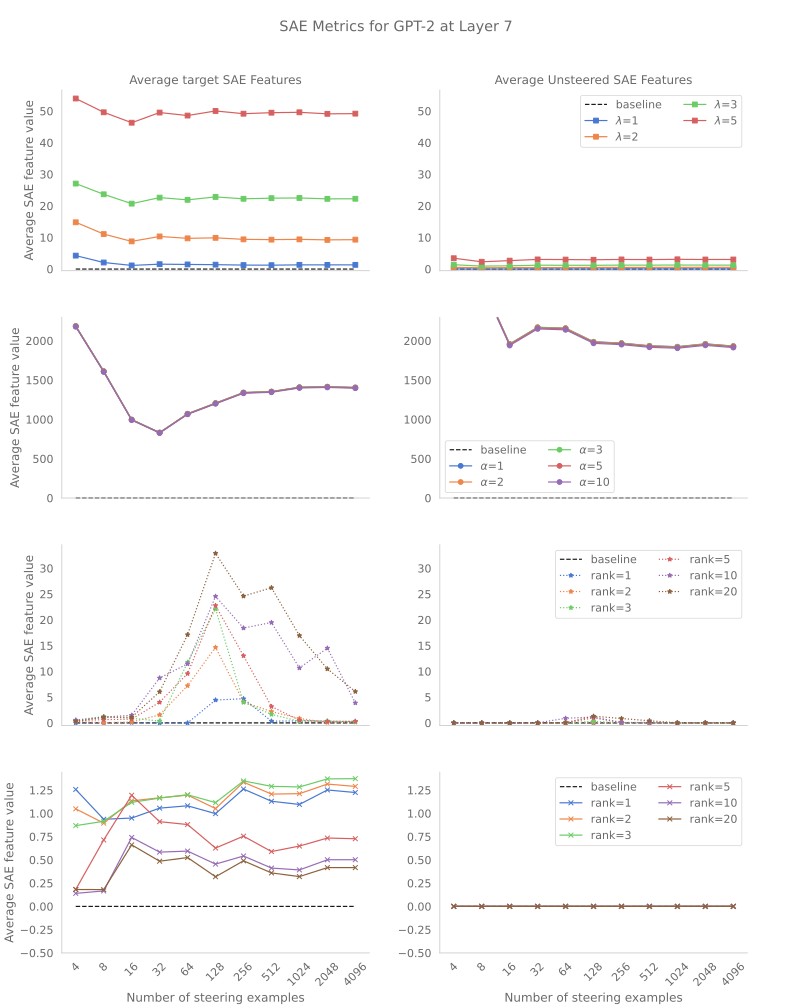
\includegraphics[width=\textwidth]{figures/gpt2_7_sae.png}
    \caption{
        The average activation of SAE features for the set of target SAE features and unsteered SAE features.
        From top to bottom the rows represent CAA \citep{caa}, ACE \citep{ace}, LoReFT \citep{reft} and LoReST \citep{steering-clear}.
        The same range of examples is used across all adaptors.
        The exact SAE feature values are only important in the unsteered case, where they should be 0, or as a comparison within the model parameters.
    \Sref{sec:prompt-pairs} describes how these metrics are calculated.}
    \label{fig:gpt-pp-sae}
\end{figure}

\begin{figure}
    \centering
    \captionsetup{width=.9\textwidth}
    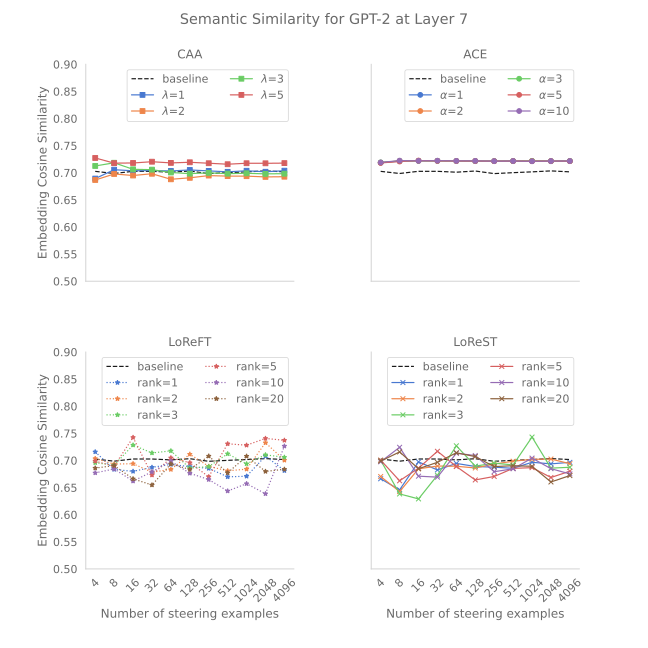
\includegraphics[width=\textwidth]{figures/gpt2_7_similarity.png}
    \caption{
        The cosine similarity of distilbert \citep{distilbert} word embeddings for the generated token.
        The number of steering examples is the same as \Fref{fig:steering-clear} and the cosine similarity is shared across charts.
        Note that the y axis has been cropped to highlight the difference between models though the change is slight.
    }
    \label{fig:gpt-pp-sim}
\end{figure}


\chapter{Conclusion}
\label{ch:conclusion}

\emph{In this chapter the analysis from the results chapter \Sref{ch:results} is drawn together into specific conclusions.}
\emph{These relate back to the contributions made in the introduction chapter \Sref{sec:contributions}.}
\emph{Important results are highlighted and their limitations discussed.}

\emph{A detailed discussion of the limitations of this project are presented.}
\emph{The effect on the conclusions drawn is highlighted.}
\emph{Finally further work that can be carried is presented.}
\emph{These directions are based on the findings of the project or areas that were not explored due to various constraints.}

\section{Limitations}

The primary limitation of the project is the compute cost and time which necessitated using GPT-2 which has a limited ability for high-level reasoning.
This means that the results of this project will not necessarily scale to modern LLMs such as Gemma \citep{gemma}, GPT-4 \citep{gpt-4}, Llama-3 \citep{llama3}, etc.
Though the results do demonstrate how steering adaptors behave in a natural language setting there is still more work to be done on quantitative analysis of steering adaptors.

Further limitations include the adaptors chosen.
The adaptors presented in this work are chosen to represent a range of steering adaptors currently proposed, however, there are many more adaptors.
Clear examples include minimally modified counterfactuals \citep{mimic} which was used in \citet{steering-clear} and probes \citep{probes}.
This project already demonstrates the wide performance range of the few commonly used adaptors, analysing the performance of more adaptors would give a better overview of representation engineering as a whole.

Finally the datasets used are small, both in the number of examples and in the number of distinct sets.
Only 5 different sets were used to generate the results in \Sref{sec:prompt-pairs-res} each with at most 3000 unique prompts.
This fails to completely capture the full range of representations that the model may contain.
Considering that the sparse autoencoder dimension for GPT-2 is 24576 \citep{saelens} 5 datasets are unlikely to encompass all concepts present in the model representation.

\section{Future Work}

Using a larger model such as Gemma \citep{gemma}, Llama 3 \citep{llama3} or GPT-5 \citep{gpt-5} (all of which have over 7 billion parameters compared to GPT-2 with 1.5 billion \citep{gpt2-1.5}) which have been instruction tuned would provide more real-world applicable results.
These models have also shown to perform far better than GPT-2 on text completion and knowledge acquisition.
With more compute it would be possible to extend the experiments in this project to these larger models.
This will also provide better analysis of affine concept editing \citep[ACE]{ace} as this method was originally developed for models such as Llama 3.

Expanding the datasets to include specific concerning behaviour present in large models (e.g. sycophancy, harmful suggestions, desire to gain more power) would provide a deeper insight into how well these adaptors may be used in practice.
Datasets such as the model written evaluations \citep[MWE]{mwe} provide a large corpus of such datasets, however, these rely on simple multiple choice questions (MCQs).
The argument for MCQs is that the possible answer tokens (``A'', ``B'' or ``yes'', ``no'') contain the full context of the question being asked \citep{steering-taxonomy}.
Potentially utilising a mixture of MCQs and free text answers can provide more insight into how best to implement steering adaptors.

Given the problems of superposition \Sref{sec:sae} that are inherent in large language models it is possible that the number of examples required to effectively steer models is larger than those presented here.
Datasets such as MWE contain only $\sim 1000$ examples and in some cases provide enough examples to effectively steer concepts \citep{steerability}.
Regardless, expanding the number of examples may provide further insight into the claims of \citet{steering-clear} about the embedding dimension, density of concepts, and number of required steering examples.

Experiments looking into the effect of the positive and negative examples would also provide more insight into the ideal choice of adaptor.
In the case of low rank methods which require explicit training it is likely that positive and negative examples need to be closely linked.
In the affine cases it may be possible to only provide positive examples to steer towards, or negative examples to steer away from.


%TC:ignore
\bibliography{references}

\appendix

\chapter{Choice of ACE Variables}
\label{app:ace}

\begin{remark}
    Recall the affine approach to steering from \cref{eq:ace}
    \begin{equation*}
        \va_\text{\normalfont steered} = \va - \text{\normalfont proj}_\vr^{\parallel}(\va) + \alpha_0\vr + \alpha\vr.
    \end{equation*}
    Given a set of positive example activations $\{\va_i^+\}_i$ and negative example activations $\{\va_i^-\}_i$ the appropriate choices for $\alpha_0$ and $\vr$ are
    \begin{equation}
        \label{eq:ace-app}
        \begin{aligned}
            \vr = \frac{1}{n}\sum_{i=1}^{n}\left(\va_i^+ - \va_i^-\right) && \alpha_0 = \text{\normalfont proj}_\vr^\parallel\left(\frac{1}{n}\sum_{i=1}^{n}\va_i^-\right)
        \end{aligned}
    \end{equation}
\end{remark}
\begin{proof}
    Let $\mu_{\va^+} = \frac{1}{n}\sum_{i=1}^{n}\va_i^+$ be the mean of the positive activations and $\mu_{\va^-}$ the mean of the negative activation.
    It is safe to assume that $\vr \in \text{span}(\mu_{\va^+} - \mu_{\va^-})$

    When $\alpha = 0$ the expected behaviour of the model should be neutral and when $\alpha = 1$ the expected behaviour should be the target behaviour.
    Therefore
    \begin{equation*}
        \begin{aligned}
            \mathbb{E}_{\alpha=0}[\va_\text{steered}] &= \mathbb{E}_\text{neutral-behaviour}[\va] = \mu_{\va^-} \\
            \mathbb{E}_{\alpha=1}[\va_\text{steered}] &= \mathbb{E}_\text{target-behaviour}[\va] = \mu_{\va^+}.
        \end{aligned}
    \end{equation*}

    Considering the first equation note that
    \begin{equation*}
        \begin{aligned}
            \mathbb{E}_{\alpha=0}[\va - \text{proj}_\vr^{\parallel}(\va) + \alpha_0\vr + \alpha\vr] &=  \mathbb{E}[\va - \text{proj}_\vr^{\parallel}(\va) + \alpha_0\vr] = \mu_{\va^-}.
        \end{aligned}
    \end{equation*}
    Taking the projection parallel to $\vr$ to both sides provides a definition for $\alpha_0$
    \begin{equation*}
        \begin{aligned}
            \text{proj}_\vr^{\parallel}(\mathbb{E}[\va - \text{proj}_\vr^{\parallel}(\va) + \alpha_0\vr]) &= \text{proj}_\vr^{\parallel}(\mu_{\va^-}) \\
            \implies \mathbb{E}[\text{proj}_\vr^{\parallel}(\va) - \text{proj}_\vr^{\parallel}(\va) + \alpha_0\text{proj}_\vr^{\parallel}(\vr)] &= \text{proj}_\vr^{\parallel}(\mu_{\va^-}) \\
            \implies \alpha_0\vr &= \text{proj}_\vr^{\parallel}(\mu_{\va^-}).
        \end{aligned}
    \end{equation*}

    Considering the second equation provides a similar result
    \begin{equation*}
        \text{proj}_\vr^{\parallel}(\mathbb{E}[\va - \text{proj}_\vr^{\parallel}(\va) + \alpha_0\vr + \vr]) = \alpha_0\vr + \vr = \text{proj}_\vr^{\parallel}(\mu_{\va^+}).
    \end{equation*}

    Subtracting these results provides a definition for $\vr$
    \begin{equation*}
        \vr = \text{proj}_\vr^{\parallel}(\mu_{\va^+}) - \text{proj}_\vr^{\parallel}(\mu_{\va^-}) = \text{proj}_\vr^{\parallel}(\mu_{\va^+} - \mu_{\va^-}).
    \end{equation*}
    As $\vr \in \text{span}(\mu_{\va^+} - \mu_{\va^-})$ the tighter bound
    \begin{equation*}
        \vr = \mu_{\va^+} - \mu_{\va^-} = \frac{1}{n}\sum_{i=1}^{n}\va_i^+ - \frac{1}{n}\sum_{i=1}^{n}\va_i^- = \frac{1}{n}\sum_{i=1}^{n}(\va_i^+ - \va_i^-)
    \end{equation*}
    is found.
    This leads to the result for $\alpha_0$ and $\vr$ in \cref{eq:ace-app}.
\end{proof}

\chapter{Prompt Pairs Dataset}
\label{app:prompt-pairs}

\chapter{{\scshape Steering Clear}: Reproduction Attempts}
\label{app:steering-clear}

\emph{The following chapter is a verbatim copy of a report that was sent to the original paper authors, \citet{steering-clear}, detailing the attempts to reproduce their work.}
\emph{The authors were quick to respond initially allowing the overall reproduction to be similar, however, they never responded to this report and the questions raised.}

\emph{The exact notation and wording is different from that used in the main thesis.}
\emph{This chapter simply contains the attempts made and associated data to demonstrate that reasonable effort was made to reproduce the exact results stated.}
\emph{Note that the dataset and model were rewritten from scratch as neither the dataset nor pre-trained model were found to be published online.}

I follow the original paper \cite{steering-clear} in all regards and any additional assumptions I make are explained below.
The paper describes the overview of how experiments were run but specific details are still missing allowing some room for interpretation.

I find that with a range assumptions across a number of trials that I am unable to fully reproduce the CAA plots the paper presents.
The primary issue I find is with the steerability metric stated in the paper, of total accuracy, where just the steered attribute accuracy results in a plot closer to the paper.

\section{Dataset}

This is a multi-label dataset:
\begin{itemize}[nolistsep]
    \item Each input is a 120 length vector representing 60 2-dimensional vectors. Each 2-dimensional vector is an ``attribute".
    \item Each label is a 60 length vector representing the target value of each of the 60 ``attributes". There are 8 target values.
    \item Each ``attribute" can take 8 values (the 8 target values) represented by a random vector from $\mathcal{N}(\mathbf{0}, \mathbf{I})$. Noise is added for each sample.
\end{itemize}

I only use $500,000$ examples rather than $2,000,000$ due to memory constraints but find that this does not affect model accuracy.
The paper does not state the exact method of generating anchor points but achieving ~100\% on the model should suffice.
I use a standard deviation of $0.01$ when adding noise to the samples thus insuring the datapoints are separable.

\section{Model}

A simple 4 layer MLP with:

\begin{itemize}[nolistsep]
    \item Layernorm after the 4 layers. This is fed into a classifier to predict the 60 labels.
    \item GeLU activation function.
    \item 512-512-256-512 hidden layer architecture.
    \item A 60 head classifier.
\end{itemize}

I test 3 types of residual streams:
\begin{itemize}[nolistsep]
    \item A single stream from input to layernorm.
    \item A residual over every single layer.
    \item No residual streams anywhere.
\end{itemize}

\begin{figure}
    \centering
    \begin{subfigure}{0.9\textwidth}
        \includegraphics[width=\textwidth]{figures/no-residual-train-curves.png}
        \caption{Train and loss curves for the MLP without any residual streams.}
        \label{fig:nr-train-curves}
    \end{subfigure}

    \begin{subfigure}{0.9\textwidth}
        \includegraphics[width=\textwidth]{figures/residual-train-curves.png}
        \caption{Train and loss curves for the MLP with a residual stream per layer.}
        \label{fig:r-train-curves}
    \end{subfigure}

    \begin{subfigure}{0.9\textwidth}
        \includegraphics[width=\textwidth]{figures/single-residual-train-curves.png}
        \caption{Train and loss curves for the MLP with a single residual stream from input to layer-norm.}
        \label{fig:sr-train-curves}
    \end{subfigure}
\end{figure}

Figures \ref{fig:nr-train-curves}, \ref{fig:r-train-curves} and \ref{fig:sr-train-curves} show the train curves for the different models.
All of these eventually reach near 100\% accuracy.
The best model is chosen based on best validation accuracy and is chosen on the first instance of the best validation loss.

\begin{figure}
    \centering
    \begin{subfigure}{0.9\textwidth}
        \includegraphics[width=\textwidth]{figures/no-residual-accuracy.png}
        \caption{The accuracy of the non-residual model on each attribute value.}
        \label{fig:nr-accuracy}
    \end{subfigure}
    \begin{subfigure}{0.9\textwidth}
        \includegraphics[width=\textwidth]{figures/residual-accuracy.png}
        \caption{The accuracy of the full residual model on each attribute value.}
        \label{fig:r-accuracy}
    \end{subfigure}
    \begin{subfigure}{0.9\textwidth}
        \includegraphics[width=\textwidth]{figures/single-residual-accuracy.png}
        \caption{The accuracy of the single residual model on each attribute value.}
        \label{fig:sr-accuracy}
    \end{subfigure}
\end{figure}

Figures \ref{fig:nr-accuracy}, \ref{fig:r-accuracy} and \ref{fig:sr-accuracy} show the accuracy of the model across all attributes and their values.
All other values are filled with a uniform random attribute.
All fills are presented to show that there is no bias towards a particular fill value.

From these plots I am fairly confident that my setup for the dataset and the training of the model is sound though there are clearly differences between how the residual streams are applied.

\section{Steering adaptor}

A forward hook is inserted at the 256-dim layer to extract activations for the contrastive pairs.
In the case of the residual stream per layer model the hook is inserted after the residual stream.

The inputs for generating the contrastive pairs are made as

\begin{itemize}[nolistsep]
    \item Selecting one attribute to target steering.
    \item Positive examples set this attribute to 0.
    \item Negative examples set this attribute to 1-7.
\end{itemize}

CAA simply takes the difference of means of these two activations as a steering vector.
A forward hook is registered at the same 256-dim layer which simply adds the scaled (parameterised by $\lambda$) steering vector to the output and returns it for the next layer.

To get repeated runs, a set of attributes is chosen\footnote{For ease of implementation these are just the first $n$ attributes} and the above process is applied to each.
In the end I run 20 repeats.

\begin{figure}
    \centering
    \includegraphics[width=0.9\textwidth]{figures/cosine-similarity.png}
    \caption{The cosine similarity between a sample of positive and negative pairs. This is for a specific attribute.}
    \label{fig:cosine-similarity}
\end{figure}

Figure \ref{fig:cosine-similarity} shows the cosine similarity of a sample of attributes.
The similarity between pairs is very high as expected as the other 59 attributes are identical.
The cross similarity is much lower showing that there is a variety of examples that are present when training the adaptor.
This plot is essentially the same across the models with minor differences in the exact similarity values.

\begin{figure}
    \centering
    \includegraphics[height=0.4\textheight]{figures/no-residual-steering.png}
    \caption{The softmax probability of the target label (0) given the input label as a function of the scaling parameter $\lambda$. This is the model without any residual streams.}
    \label{fig:nr-steering}
\end{figure}

\begin{figure}
    \centering
    \includegraphics[height=0.4\textheight]{figures/residual-steering.png}
    \caption{The softmax probability of the target label (0) given the input label as a function of the scaling parameter $\lambda$. This is the model with a residual streams per layer.}
    \label{fig:r-steering}
\end{figure}

\begin{figure}
    \centering
    \includegraphics[height=0.4\textheight]{figures/single-residual-steering.png}
    \caption{The softmax probability of the target label (0) given the input label as a function of the scaling parameter $\lambda$. This is the model with a single residual stream from input to layernorm.}
    \label{fig:sr-steering}
\end{figure}

Figures \ref{fig:nr-steering}, \ref{fig:r-steering} demonstrate the effect of the CAA steering on the different attribute values for the target attribute.
The remaining attribute values are randomly selected.
The experiment is run over a range of example values for each 20 repeats and for each experiment the mean over 100 test inputs is returned.

Clearly demonstrated is that 4 and 8 examples do not achieve the same efficacy as the other examples regardless of the strength of the steering vector.
This does not take into account the effect on the attributes nor the softmax prob of the other values.
These experiments demonstrate that the steering vectors are able to steer effectively.

\section{Steering metric}

A subset of 1000 of the contrastive pairs above are withheld during training.
The negative generating inputs are fed through the model with the trained steering adaptor and the output recorded.
The goal is for the output to match the positive generating labels.

There are two metrics that I test:
\begin{itemize}[nolistsep]
    \item The accuracy on the steered attribute alone.
    \item The accuracy on all the attributes (this is the one stated in the paper).
\end{itemize}

\begin{figure}
    \centering
    \begin{subfigure}{0.45\textwidth}
        \includegraphics[width=\textwidth]{figures/no-residual-reproduction.png}
        \caption{Standard model steering accuracy on the steered attribute alone.}
        \label{fig:nr-reproduction}
    \end{subfigure}
    \hfill
    \begin{subfigure}{0.45\textwidth}
        \includegraphics[width=\textwidth]{figures/residual-reproduction.png}
        \caption{Residual model steering accuracy on the steered attribute alone.}
        \label{fig:r-reproduction}
    \end{subfigure}
    \begin{subfigure}{0.45\textwidth}
        \includegraphics[width=\textwidth]{figures/single-residual-reproduction.png}
        \caption{Single residual stream model steering accuracy on the steered attribute alone.}
        \label{fig:sr-reproduction}
    \end{subfigure}
\end{figure}

Figures \ref{fig:nr-reproduction}, \ref{fig:r-reproduction} and \ref{fig:sr-reproduction} show the attempt at reproducing the paper figures for the top-left plot in Figure 1.
This only focuses on the CAA approach.
This uses a different metric to the paper focusing only on attribute accuracy rather than total accuracy and the trends are similar to those in the paper.
However, these plots are still not the same as the papers plots especially as they do not use the same metric.

\begin{figure}
    \centering
    \begin{subfigure}{0.45\textwidth}
        \includegraphics[width=\textwidth]{figures/no-residual-full-reproduction.png}
        \caption{Standard model steering accuracy on the steered attribute alone.}
        \label{fig:nr-correct}
    \end{subfigure}
    \hfill
    \begin{subfigure}{0.45\textwidth}
        \includegraphics[width=\textwidth]{figures/residual-full-reproduction.png}
        \caption{Residual model steering accuracy on the steered attribute alone.}
        \label{fig:r-correct}
    \end{subfigure}
    \begin{subfigure}{0.45\textwidth}
        \includegraphics[width=\textwidth]{figures/single-residual-full-reproduction.png}
        \caption{Single residual stream model steering accuracy on the steered attribute alone.}
        \label{fig:sr-correct}
    \end{subfigure}
\end{figure}

Figures \ref{fig:nr-correct}, \ref{fig:r-correct} and \ref{fig:sr-correct} show the reproduction using the stated steering metric of total accuracy across all target labels.

\chapter{Layer Sweeps}

\emph{This chapter includes the figures generated when running the experiments across all 11 layers of GPT-2 small \citep{saelens}.}
\emph{It is important to note that the exact metrics presented in \cref{sec:prompt-pairs} are not used here.}
\emph{Instead the absolute SAE activation values are used to better get a sense of how strongly the adaptors are effecting the model.}

\emph{Only CAA is presented here as a proxy for the other runs and to save pages.}
\emph{The ideal choice of layer was found to be layer 7, discussion of the figures will not be carried out due to the number of figures presented.}

\begin{figure}
    \centering
        \includegraphics[width=\textwidth]{figures/gpt2_sweep_0.png}
        \label{fig:0}
\end{figure}

\begin{figure}
    \centering
        \includegraphics[width=\textwidth]{figures/gpt2_sweep_1.png}
        \label{fig:1}
\end{figure}

\begin{figure}
    \centering
        \includegraphics[width=\textwidth]{figures/gpt2_sweep_2.png}
        \label{fig:2}
\end{figure}

\begin{figure}
    \centering
        \includegraphics[width=\textwidth]{figures/gpt2_sweep_3.png}
        \label{fig:3}
\end{figure}

\begin{figure}
    \centering
        \includegraphics[width=\textwidth]{figures/gpt2_sweep_4.png}
        \label{fig:4}
\end{figure}

\begin{figure}
    \centering
        \includegraphics[width=\textwidth]{figures/gpt2_sweep_5.png}
        \label{fig:5}
\end{figure}

\begin{figure}
    \centering
        \includegraphics[width=\textwidth]{figures/gpt2_sweep_6.png}
        \label{fig:6}
\end{figure}

\begin{figure}
    \centering
        \includegraphics[width=\textwidth]{figures/gpt2_sweep_7.png}
        \label{fig:7}
\end{figure}

\begin{figure}
    \centering
    \includegraphics[width=\textwidth]{figures/gpt2_sweep_8.png}
    \label{fig:8}
\end{figure}

\begin{figure}
    \centering
        \includegraphics[width=\textwidth]{figures/gpt2_sweep_9.png}
        \label{fig:9}
\end{figure}

\begin{figure}
    \centering
        \includegraphics[width=\textwidth]{figures/gpt2_sweep_10.png}
        \label{fig:10}
\end{figure}

\begin{figure}
    \centering
    \includegraphics[width=\textwidth]{figures/gpt2_sweep_11.png}
    \label{fig:11}
\end{figure}

%TC:endignore

\end{document}
